\chapter{Creating a data split}

In this chapter we will describe the data set used throughout the thesis. The
process used to select the split between training, testing and validation
data is also described.

\section{Data set}

The ASK corpus (\emph{andrespråkskorpus}) was presented in 2006
\autocite{tenfjord06}. The corpus contains Norwegian learner essays from two
different language tests: \emph{Språkprøven i norsk for voksne innvandrere}
and \emph{Test i norsk – høyere nivå}, which test proficiency at the B1 and
B2 levels, respectively. Following the naming in
\textcite{carlsen2012proficiency}, we will refer to these tests as the
\emph{IL test} (Intermediate Level, ``Språkprøven'') and the \emph{AL test}
(Advanced Level, ``Høyere nivå'').

\begin{table}
  \centering
  \begin{tabular}{lrrr}
    \toprule
    First language             & AL test & IL test & Total \\
    \midrule
    English                    &     100 &     100 &   200 \\
    Polish                     &     100 &     100 &   200 \\
    Russian                    &     100 &     100 &   200 \\
    Somali                     &       7 &     100 &   107 \\
    Spanish                    &     100 &     100 &   200 \\
    German                     &     100 &     100 &   200 \\
    Vietnamese                 &       5 &     100 &   105 \\
    \midrule
    Subtotal (included languages) &  512 &     700 &  1212 \\ \addlinespace
    \midrule
    (Albanian)                 &      24 &     100 &   124 \\
    (Bosnian-Croatian-Serbian) &     100 &     100 &   200 \\
    (Dutch)                    &     100 &     100 &   200 \\
    (Norwegian nynorsk)        &      21 &      11 &    32 \\
    (Norwegian bokmål)         &      79 &      89 &   168 \\
    \midrule
    Subtotal (excluded languages) &  324 &     400 &   724 \\ \addlinespace
    \midrule
    Total (all languages)      &     836 &    1100 &  1936 \\
    \bottomrule
  \end{tabular}
  \caption{Texts in each test level for all \acp{L1}.
           Excluded languages are listed in round brackets.}
  \label{tab:l1-and-testlevel}
\end{table}

The corpus contains 1736 texts\footnote{In
\textcite{carlsen2012proficiency,malmasi15,malmasi17}, it's reported that it
contains 1700 texts.}. Each document includes metadata such as the writer's
L1: one of German, Dutch, English, Spanish, Russian, Polish,
Bosnian-Croatian-Serbian, Albanian, Vietnamese and Somali. All texts from
seven of these language backgrounds, 1212\footnote{Reported to be 1222 in
\textcite{carlsen2012proficiency}.} in total, have been assigned a \ac{CEFR}
score, and these texts comprise the subcorpus we will be working with. In
particular, all texts except those written by people with Dutch,
Bosnian-Croatian-Serbian or Albanian as L1 have a CEFR score. The CEFR labels
are available since work by \textcite{carlsen2012proficiency}, and were not
included at the corpus' initial release. Table \ref{tab:l1-and-testlevel}
shows the number of texts in the corpus for each native language and at each
test level.

Among the languages we include, there are five languages from the
Indo-European language family. Breaking them further down into branches,
there are two Germanic (English and German), two Slavic (Polish and Russian),
and one Italic language, Spanish. Finally, there is one Afro-Asiatic
language, Somali, and one Austroasiatic, Vietnamese.

The corpus also includes 200 texts written by native Norwegian speakers as a
control corpus, bringing the total number of documents up to 1936. The total
number of word and punctuation tokens in the full corpus, including the
control corpus, is approximately 770,000. Restricting the corpus to the 1212
documents with \ac{CEFR} score, the number of tokens is approximately 487,000
in total. Other metadata, apart from L1 and CEFR score, includes, but are not
limited to: the test level the essay was written for, what topic the essay
is about, and the learner's country of origin, age, and gender.

The CEFR scores in the ASK corpus range between A2 and C1, and also includes
intermediate labels between the canonical proficiency scores, such as A2/B1
and B1/B2. Thus, the total number of distinct CEFR scores is seven, which is
more fine-grained than the TOEFL11 corpus \autocite{blanchard13}, which only
uses three distinct proficiency categories, or the corpus used in
\textcite{vajjala18universalCEFR}, the MERLIN corpus, where the CEFR scores
range between A1 and C1, but without any intermediate levels.

The fine-grained labels makes it challenging to train and evaluate models,
and also to compare the results against work on other corpora, because the
gravity of a misclassification may not the same on the more fine-grained
labels.
 

\subsection{Analyzing non-linguistic variables}

\begin{figure}
  \centering
  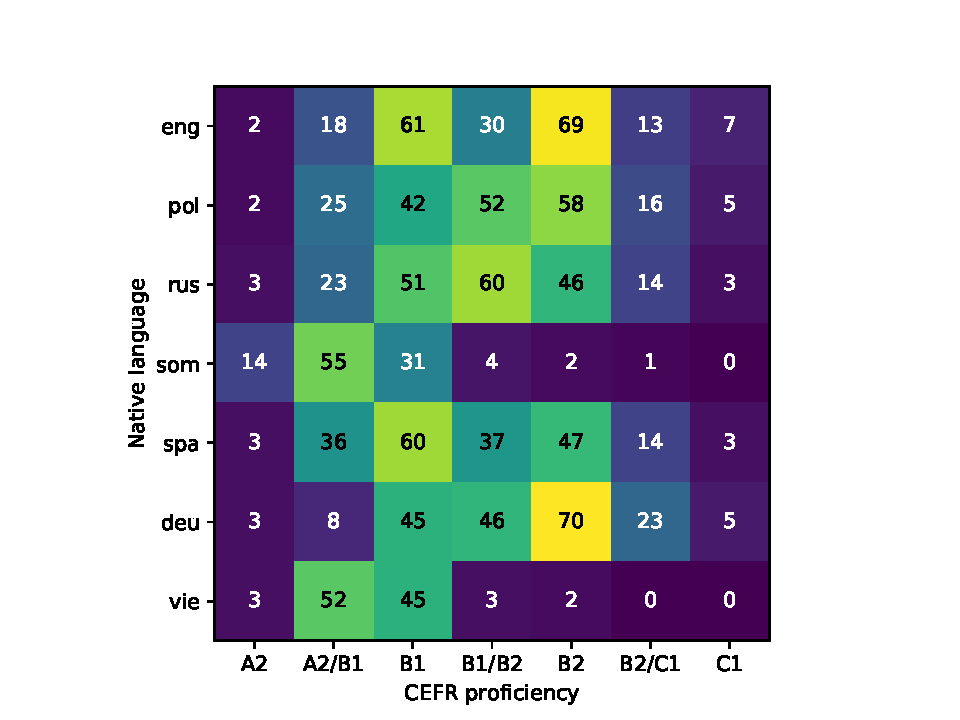
\includegraphics[height=0.3\textheight]{lang_vs_cefr}
  \caption{The distribution of proficiency scores for each L1}
  \label{fig:lang-vs-cefr}
\end{figure}
 
\begin{figure}
  \centering
  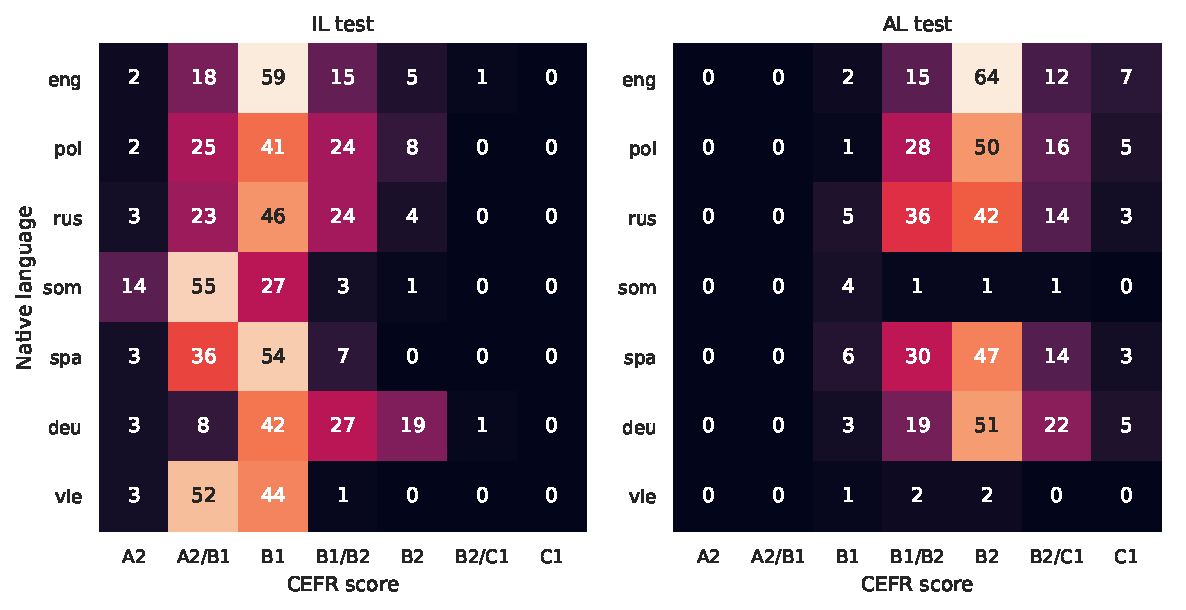
\includegraphics[width=\textwidth]{testlevel_lang_vs_cefr}
  \caption{L1 versus CEFR score for each test level}
  \label{fig:testlevel-lang-vs-cefr}
\end{figure}

Analysis of the data set was carried out in order to find correlations
between different metadata. Knowing that the documents stem from two
different language tests that measure different levels of proficiency, the
data set was split in two using the \emph{Test level} label, and then broken
down by language and proficiency again. Figure \ref{fig:testlevel-lang-vs-cefr}
shows that the test levels have different distributions of proficiency. Note
also that two language groups are underrepresented at the B2 test level
(\emph{AL test}), namely Somali and Vietnamese, which have seven and five
essays in the B2 test level, respectively. All other combinations of L1 and
test level contain exactly 100 essays. This partly explains the low average
proficiency of Somali and Vietnamese speakers apparent in figure
\ref{fig:lang-vs-cefr}. The difference compared to the other language groups is
not as salient when looking only at the B1 test level (\emph{IL test}) data.

\begin{table}
  \centering
  \begin{tabular}{lrrr}
    \toprule
    Topic                    & AL test & IL test & Total \\
    \midrule
    telefon                  &      37 &      64 &   101 \\
    bolig                    &       0 &      83 &    83 \\
    familie helse vekt       &      59 &       0 &    59 \\
    tid                      &       2 &      51 &    53 \\
    natur norge              &       0 &      48 &    48 \\
    folk relasjoner vennskap &       0 &      45 &    45 \\
    tradisjoner flytting     &       0 &      38 &    38 \\
    barn                     &       3 &      32 &    35 \\
    kultur norge             &       0 &      34 &    34 \\
    media                    &       0 &      31 &    31 \\
    \bottomrule
  \end{tabular}
  \caption{Number of texts in each test level for top 10 topics}
  \label{tab:texts-per-topic}
\end{table}

Another interesting variable is the essay topic. There is generally a strong
correlation between topic and vocabulary, and not accounting for this may
lead to a model picking up the wrong signal. Since the data is collected from
two different language tests, we might expect the distribution of topics to
differ between the test levels, and this is the case. Looking at the ten most
common topics in the data (table \ref{tab:texts-per-topic}), several are only
present on one test level.

There is also a difference in granularity. There are 52 topics in ``Høyere
nivå'' and only 38 topics in \emph{IL test}, even though there are more
documents in the latter test level (512 vs. 700). This also means that the
topics within each test level have different support. The median number of
documents for a topic in \emph{AL test} is 5 (mean $9.8$), while it is 11 in
\emph{IL test} (mean $18.4$). This also explains the overrepresentation of
\emph{IL test} in the table of top ten topics.

It has been observed that some topics in the diagram consist of several
sub-topics (for instance, ``natur norge'' consists of ``natur'' and
``norge''). However, the number of individual sub-topics is 62, still quite
large. However, they seem to be more evenly distributed across essays. The
median number of documents for a sub-topic, for both test levels, is 25 (mean
$34.8$). 13 sub-topics are only represented in 5 or fewer documents.

\begin{figure}
  \centering
  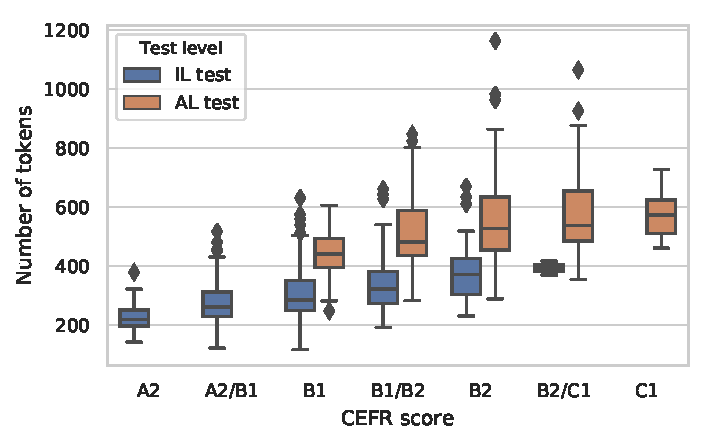
\includegraphics[width=\textwidth]{testlevel_lengths_per_cefr}
  \caption{Distributions of essay lengths for CEFR scores on each test level}
  \label{fig:testlevel-lengths-per-cefr}
\end{figure}

Document lengths have been seen to correlate with essay score in other
studies such as \textcite{vajjala17}. To see the relationship between these
variables in ASK, we again break down the data into the two test levels. One
group, \emph{B2/C1} CEFR score within \emph{IL test}, was excluded due to
having fewer than ten documents. Looking at figure
\ref{fig:testlevel-lengths-per-cefr}, two relations are apparent. Essays in the
\emph{AL test} test level are generally longer than in \emph{IL test}, and
within each test level the higher scoring essays are generally longer.
Also, outliers are generally on the long side.

Note that even for the same CEFR score, the essays from the higher test level
are considerably longer. As an example, consider the \emph{B1/B2} score,
which is the most evenly distributed between the two test levels (101 essays
in \emph{IL test}, 131 in \emph{AL test}). More than 75\% of these texts on
the lower test level have fewer than 400 tokens, and more than 75\% on the
higher level are longer than 400 tokens. In fact, for all four CEFR scores
that are present on both test levels, there is no overlap of the
interquartile ranges\footnote{The range of values when the top 25\% and
bottom 25\% are excluded} between IL and AL test level.


\subsection{Data split}

At the start of the project, the dataset was split into a training,
development and test set in a 8:1:1 proportion. Ideally, the train and test
sets would have the same distribution of classes, but the limited amount of
data made this more difficult. As can be seen from figure \ref{fig:lang-vs-cefr},
15 of the combinations language vs. proficiency label consist of only three
or fewer documents.

Moreover, we wanted each split to consist of text topics not present in the
other splits. The reason for this to prevent a model from learning a bias for
topic. Finding a split that satisfies our constraints is an optimization
problem for which it can be intractable to find an optimal solution. We
therefore turned to heuristics, hoping that it would help us find a good
local optimum.
 
The split was chosen in order to have the right proportion of documents in
each part of the split, and so the distribution of proficiency and native
language is as similar as possible across the separate parts of the data
split. Specifically, the split was found by running an evolutionary algorithm
with a fitness function favouring splits that were as close as possible to
8:1:1 in proportion, while maintaining a low Kullback-Leibler divergence of
the proficiency and language distributions against the entire corpus.

\begin{table}
  \centering
  \begin{tabular}{ll}
    \toprule
    Topics in development set &       Topics in test set \\
    \midrule
         idrett/sport kultur &       geografi norge folk \\
                organisasjon &               innvandring \\
                  opplevelse & innvandring politikk valg \\
                     økonomi &              idrett/sport \\
                    holdning &            bolig geografi \\
           barn idrett/sport &               arbeid yrke \\
            familie flytting &          økonomi holdning \\
               eldre familie &              humor kultur \\
               helse røyking &   politikk norge holdning \\
       litteratur dikt språk &            litteratur bok \\
    helse arbeid innvandring &  familie befolkning norge \\
                barn familie &    litteratur dikt idrett \\
                       helse &           folk utdannelse \\
            utdannelse språk &         politikk holdning \\
          arbeid innvandring &                  media tv \\
      litteratur dikt venner &                  religion \\
                             &               helse organ \\
                             &             folk følelser \\
    \bottomrule
  \end{tabular}
  \caption{The topics chosen to be in each of the development and test sets}
  \label{tab:topics-in-split}
\end{table}

The split in terms of the topics can be seen in table \ref{tab:topics-in-split}.
The dev and test sets contain 123 texts each. The topic variable has values
which are sets of keywords, and therefore there is still topical overlap
between splits. For example, ``økonomi'' (economy) and ``økonomi holdning''
(economy attitude) are considered separate values and assigned to different
splits, even though both topics include the economy keyword.
